\documentclass[letterpaper]{article}
\usepackage[margin=1in]{geometry}
\usepackage[utf8]{inputenc}
\usepackage{textcomp}
\usepackage{amssymb}
\usepackage{natbib}
\usepackage{graphicx}
\usepackage{gensymb}
\usepackage{amsthm, amsmath, mathtools}
\usepackage[dvipsnames]{xcolor}
\usepackage{enumerate}
\usepackage{mdframed}
\usepackage[most]{tcolorbox}
\usepackage{csquotes}
% https://tex.stackexchange.com/questions/13506/how-to-continue-the-framed-text-box-on-multiple-pages

\tcbuselibrary{theorems}

\newcommand{\R}{\mathbb{R}}
\newcommand{\Z}{\mathbb{Z}}
\newcommand{\N}{\mathbb{N}}
\newcommand{\Q}{\mathbb{Q}}
\newcommand{\C}{\mathbb{C}}
\newcommand{\code}[1]{\texttt{#1}}
\newcommand{\mdiamond}{$\diamondsuit$}
\newcommand{\PowerSet}{\mathcal{P}}
\newcommand{\Mod}[1]{\ (\mathrm{mod}\ #1)}
\DeclareMathOperator{\lcm}{lcm}

%\newtheorem*{theorem}{Theorem}
%\newtheorem*{definition}{Definition}
%\newtheorem*{corollary}{Corollary}
%\newtheorem*{lemma}{Lemma}
\newtheorem*{proposition}{Proposition}


\newtcbtheorem[number within=section]{theorem}{Theorem}
{colback=green!5,colframe=green!35!black,fonttitle=\bfseries}{th}

\newtcbtheorem[number within=section]{definition}{Definition}
{colback=blue!5,colframe=blue!35!black,fonttitle=\bfseries}{def}

\newtcbtheorem[number within=section]{corollary}{Corollary}
{colback=yellow!5,colframe=yellow!35!black,fonttitle=\bfseries}{cor}

\newtcbtheorem[number within=section]{lemma}{Lemma}
{colback=red!5,colframe=red!35!black,fonttitle=\bfseries}{lem}

\newtcbtheorem[number within=section]{example}{Example}
{colback=white!5,colframe=white!35!black,fonttitle=\bfseries}{def}

\newtcbtheorem[number within=section]{note}{Important Note}{
        enhanced,
        sharp corners,
        attach boxed title to top left={
            xshift=-1mm,
            yshift=-5mm,
            yshifttext=-1mm
        },
        top=1.5em,
        colback=white,
        colframe=black,
        fonttitle=\bfseries,
        boxed title style={
            sharp corners,
            size=small,
            colback=red!75!black,
            colframe=red!75!black,
        } 
    }{impnote}
\usepackage[utf8]{inputenc}
\usepackage[english]{babel}
\usepackage{fancyhdr}
\usepackage[hidelinks]{hyperref}

\pagestyle{fancy}
\fancyhf{}
\rhead{POLI 112A}
\chead{Thursday, January 12, 2023}
\lhead{Lecture 1}
\rfoot{\thepage}

\setlength{\parindent}{0pt}

\begin{document}

\section{Introduction (Chapter 1 \& 2)}
In this class, our goal is to understand politics (i.e., the causes and mechanisms). The only problem is that the political world is complicated. Observing events is simply not enough to understand what is going on and why. Therefore, the solution is to represent reality in a simplifed way, allowing us to focus on the most relevant elements. This is known as the \emph{theoretical models of politics.}

\subsection{Models}
A model is
\begin{itemize}
    \item a \textbf{simplified representation}. 
    \item \emph{not} exact pictures of the real world.
\end{itemize}
In other words, we can think of a model as a \emph{map} -- we only need to focus on what is relevant. Thus, it's necessary to simplify the model to isolate variables of interest and be able to ``navigate.''

\subsection{Theoretical Models of Politics}
A model gives a stylized representation that identifies, or makes assumptions about, the key ingredients of a political phenomenon. Generally speaking, a model contains information about  
\begin{itemize}
    \item the key actors involved. 
    \item their objectives. 
    \item strategic choices they are faced with. 
\end{itemize}
For example, if we wanted to talk about winning elections, then 
\begin{itemize}
    \item the key actors could be the different parties (Republicans and Democrats).
    \item the objectives could be winning elections. 
    \item the strategic choices could be which candidate the parties could support in the primary elections.
\end{itemize}
Once we have this stylized representation, the model allows us to propose an explanation for an empirical pattern, or the mechanisms underlying a phenomenon. 

\bigskip 

Assumptions lead us to conclusions about how, why, and when political actors behave. In other words, conclusions are predictions of
\begin{itemize}
    \item what is going to happen? 
    \item how will the key actors behave in key $X$ or $Y$? 
\end{itemize}

\subsection{Rationality: the Model of Choice}
The key assumption\footnote{The underlying rational choice theory.} we'll make is that political actors\footnote{Literally anyone interested in politics.} are instrumentally rational. They have consistent preferences and act in accordance to them. 

\subsubsection{Preferences}
An individual's preferences determine the value they attach to different alternatives or outcomes. For example, a voter has preference over political parties.

\bigskip 

If a voter prefers Democrats over Republicans, that voter gets a higher \textbf{value} (\textbf{payoff}/\textbf{utility}) from a Democrat being elected. 

\subsubsection{Consistent Preferences}
Individual preferences are consistent if they are 
\begin{itemize}
    \item complete: either I prefer Democrats ($D > R$) or Republicans ($R > D$), or I am indifferent\footnote{It's okay to be indifferent, but not knowing is not allowed in this context.} ($D = R$).
    \item transitive: if I prefer candidate $A$ to candidate $B$, and candidate $B$ to candidate $C$, then I prefer $A$ to $C$. 
\end{itemize}


\subsubsection{Instrumental Rationality}
Suppose there is certainty over how different actions map into different outcomes or alternatives (i.e., you know how your actions will affect the resulting value). 

\bigskip 

An \textbf{instrumentally rational individual} simply takes the action that leads to their preferred outcome (i.e., the outcome associated with the highest value).

\bigskip 

This is associated with \emph{certainty}: you should know exactly how the different possible actions can translate to different possible outcomes. For example, as a \emph{single voter} (i.e., if your vote alone could elect anyone), then if the single voter picks a Democrat, then we'll have a Democrat. This is a \emph{certain} outcome. 

\subsubsection{Expected Utility}
When individuals face uncertainty\footnote{Not knowing how your actions will affect your utility} over the consequences of their actions, instrumental rationality is not so easy to apply.

\bigskip 

Therefore, to handle the situations of uncertainty, we must define the concept of \emph{expected utility}.

\subsubsection{Example of Expected Utility}

    Suppose you are a potential independent candidate choosing whether to run for office in the next election. You care about policies that will be implemented by elected representatives (you do not care about just winning.)

    \bigskip 

    For obvious reasons, you prefer your own policies, but you like the Democratic candidate's policies better than the Republican's policies. 

    \bigskip 

    Therefore, you assign a value of \textbf{100} to your own policies, \textbf{50} to the Democratic candidate's policy, and \textbf{10} to the Republican candidate's policy. 

    \bigskip 

    You must think about how your actions (entering the race or staying home) influences the outcome of the election. \textbf{The issue is that you do not know, for sure, who is going to win.} What should you do? What is the optimal course of action (i.e., what maximizes your expected utility)?

\begin{mdframed}
    Recalling that the goal is to maximize our utility, we want to devise a formula that can be used to determine the expected utility. One way to do this is to create a formula that assigns weight using probability. One such formula could be
    \[EU(R) = 100 \cdot \PR_{I}(R) + 50 \cdot \PR_{D}(R) + 10 \cdot \PR_{R}(R),\]
    where 
    \begin{itemize}
        \item $EU(R)$ is a function that takes in $R$, the event that you run, and returns the expected utility.
        \item $\PR_{I}(R)$ is the probability that you win, 
        \item $\PR_{D}(R)$ is the probability that the Democratic party wins if you run, and 
        \item $\PR_{R}(R)$ is the probability that the Republican party wins if you run. 
    \end{itemize} 
    It should come as no surprise that 
    \[\PR_{I}(R) + \PR_{D}(R) + \PR_{R}(R) = 1.\]
    Therefore, 
    \[EU(NR) = 100 \cdot 0 + 50 \cdot \PR_{D}(R) + 10 \cdot \PR_{R}(R),\]
    where 
    \begin{itemize}
        \item $EU(NR)$ is a function that takes in $NR$, the event that you do not run, and returns the expected utility, and 
        \item $100 \cdot 0$ comes from the fact that, if you do not run, the probability that you run from running must be 0.
    \end{itemize}
    Therefore, to decide your best course of action, you must consider the probability of each candidate winning if you enter the race, and if you do not (e.g., consider the polls). Given the probabilities, and the values attached to each candidate's policies, you can calculate the expected utility of running and the expected utility of staying home. 

    \bigskip 

    Instrumental rationality implies that you should take the action that gives you the \textbf{higher} expected utility (optimal, in expectation).

    \bigskip 

    Suppose that you choose to stay home. Suppose further that 
    \begin{itemize}
        \item Democrats win with probability $0.6$,
        \item Republicans win with probability $1 - 0.6 = 0.4$.
    \end{itemize}
    The expected utility of staying home is therefore 
    \[0.4 \cdot 10 + 0.6 \cdot 50 = \boxed{34}.\]

    Suppose that you choose to run. Suppose further that 
    \begin{itemize}
        \item You win with probability $0.2$,
        \item Democrats win with probability $0.3$,
        \item Republicans win with probability $0.5$. 
    \end{itemize}
    The expected utility of running is 
    \[0.5 \cdot 10 + 0.3 \cdot 50 + 0.2 \cdot 100 = \boxed{40}.\]

    The ``rational'' action (i.e., the one that maximizes your expected utility) is entering the race. In expectation, \emph{this leaves you better off, even if you know that, by running, you are increasing the probability of your least preferred candidate winning the election.}
\end{mdframed}

\subsubsection{Rationality}
We should note that rationality in this course 
\begin{itemize}
    \item is acting in accordance to one's own consistent preferences\footnote{Given your goals, are you acting in your own best interest?} (instrumental).
    \item is \textbf{not} acting in accordance to normative or moral principles\footnote{We don't care about why someone has their preferences}.
    \item is \textbf{not} acting on economic self-interest\footnote{Being rational is not the same as being selfish or selfless}.
\end{itemize}
The concept of instrumental rationality does not contain a normative judgement about an individual's actions or objectives.
% page 46































\newpage
\section{Elections and Ideology (Chapter 5)}
Our focus is in elections as ideological contests: parties compete in elections by proposing different policy platforms. Voters support the party that proposes the policies that they like the most (i.e., the one that most closely aligns to their ideology). 

\bigskip 

Therefore, the questions we want to focus on are:
\begin{itemize}
    \item What platforms will political parties propose? 
    \item Should parties moderate, or go to the extremes? 
    \item Do ideological parties propose more extreme policies than electorally motivated ones?
\end{itemize}

\subsection{Modeling Voters' Ideology}
Voters' ideology determines their policy preferences (i.e., the value, or payoff/utility, they attach to different policy platforms). We can represent the various policies as numbers along a line, known also as the \emph{ideological continuum}.
\begin{center}
    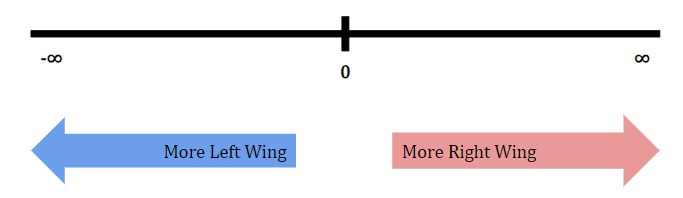
\includegraphics[scale=0.9]{assets/continuum.png}
\end{center}
As seen, low numbers are left-wing policies and high numbers are right-wing policies.

\subsection{Ideology as a Single-Peaked Preference}
Each voter has a preferred policy, represented by a point along the line. Generally, voters like policies that are \emph{close} to their preferred point. 

\bigskip

Their \textbf{policy utility}, or the value voters attach to the different policy alternatives, is highest at their preferred point, and decreases as the policy moves away from this point. If we imagine this as a graph, the voters' policy preferences are \emph{single-peaked}\footnote{The one point the voter wants the most.}\footnote{The curve does not need to be symmetrical.}.

\subsubsection{Example: Graphical Representation}
Consider the following graph, where the $x$-axis is the \textbf{utility} and the $y$-axis is the \textbf{policy utility}.
\begin{center}
    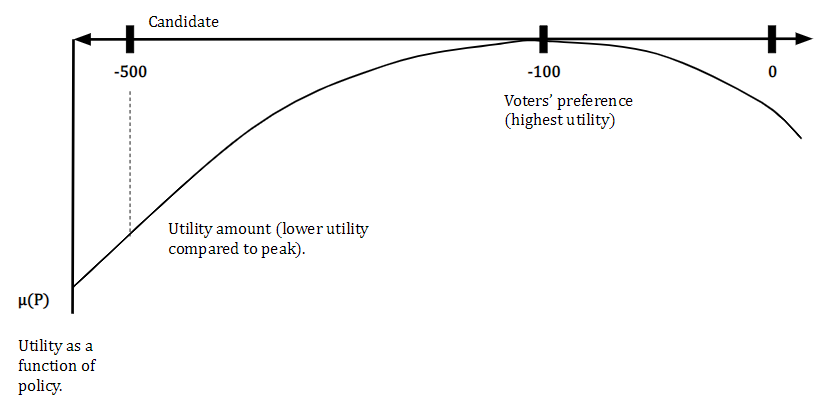
\includegraphics[scale=0.9]{assets/ideology_peak.png}
\end{center}
Here, the single peak is at $-100$ since this is the \emph{ideal policy}. If we pick the candidate's policy, we would end up with a lower policy utility than if we picked the preferred policy. 

\subsubsection{Example: Non-Single Peaked Preference - Graphical Representation}

\begin{center}
    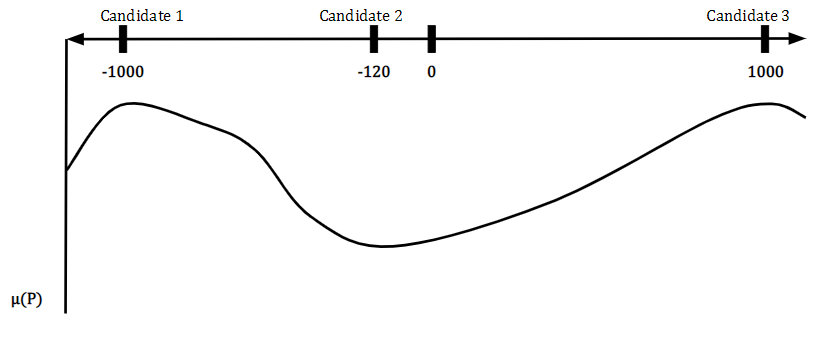
\includegraphics[scale=0.8]{assets/ideology_non_single_peak.png}
\end{center}

In this example there are two peaks -- one for candidate 1 and the other has candidate 3. The idea is that two extremes could end up converging (e.g., someone who's very left-wing may prefer someone who's very right-wing than a moderate).

\subsection{Black's Median Voter Theorem}
Suppose voters have single-peaked preferences. Then, the ideal point of the median voter is the majority-preferred policy (i.e., \textbf{it beats all other alternatives} in pairwise comparisons). This is known as the \textbf{condorcet winner} -- people will vote for those closest to their ``peak'' (i.e., majority wins).

\bigskip 

The \textbf{median voter} (MV) is the voter whose preferred policy ``splits'' the electorate in half; that is, half of all voters has preferred point to the left of the median voter, and half of all voters has preferred point to the right. 

\bigskip 

The idea behind this theorem is that 50\% of all voters prefer policy on the left, and 50\% of all voters prefer policy on the right of the MV. Single peakness implies that the median voter's views is the majority. 
\begin{center}
    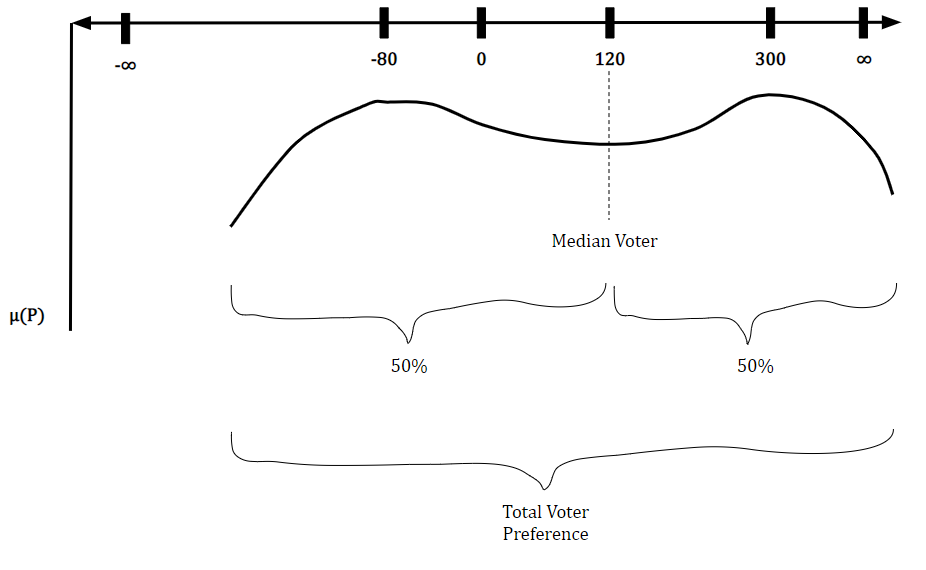
\includegraphics[scale=0.7]{assets/black_thm_proof.png}
\end{center}
% 96 (109 in pdf)

\subsection{Electoral Competition}
Now that we know how to represent voters' ideology (i.e., their preferences over the policy space), we can go back to the original question mentioned at the beginning of the section: 
\begin{mdframed}
    \begin{itemize}
        \item What platforms will political parties propose? 
        \item Should parties moderate, or go to the extremes? 
        \item Do ideological parties propose more extreme policies than electorally motivated ones?
    \end{itemize}
\end{mdframed}

\subsubsection{A Formal Model}
For electoral competition, there are several ingredients of a model: 
\begin{itemize}
    \item Who the key actors are 
    \item What their goals are 
    \item What strategic choices they are faced with 
\end{itemize}

\subsubsection{Downsian Economic Theory of Democracy}
The ingredients of the Downsian model of elections are 
\begin{itemize}
    \item Two parties, $L$ and $R$ 
    \item Each party chooses a policy platform represented by a number along the real line $-\infty$ to $\infty$ (i.e., extreme left to extreme right)
    \item Parties care about winning elections (office seeking)
    \item Voters have single peaked preferences over policy platforms (i.e., prefer policies closer to their preferred point)
    \item The party that wins most votes wins the election. If tied, each wins with probability $\frac{1}{2}$. 
\end{itemize}

\subsubsection{Applying Downsian to Tweedledum and Tweedledee}
Suppose voter preferences are single-peaked. Then, under any distribution of the voters' preferences, both parties will propose the ideal policy of the median voter (full convergence).

\bigskip 

Strategic parties interested in \emph{solely winning elections} will have no reason to polarize. Their strategic incentives will always push both of them towards ``moderate'' positions; they will always converge on the preferred platform of the median voter. 

\subsubsection{Visualization}
If you get \emph{closer} to the MV, you are more likely to win. If you move \emph{away} from the MV, you will basically lose. Therefore, the idea is that both parties will converge to the MV. 
\begin{itemize}
    \item Here, $R$ will win because it is the closest to the MV. In the above line, the MV is \emph{aligned} with the views of the MV whereas the $L$ isn't. In the below line, $R$ is \emph{closer} to the MV than $L$ is, so $R$ will again win. 
    \begin{center}
        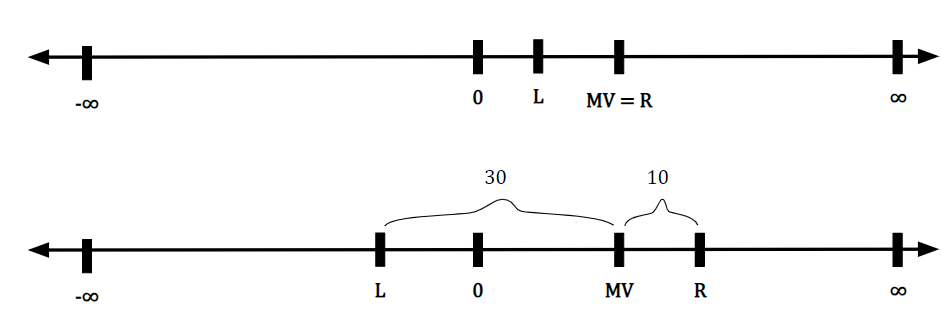
\includegraphics[scale=0.6]{assets/downsian_2.png}
    \end{center}

    \item The idea is that there will be a \emph{tie} if both groups converge on the same number, or if both groups are \emph{equidistant} from the the MV. 
    \begin{center}
        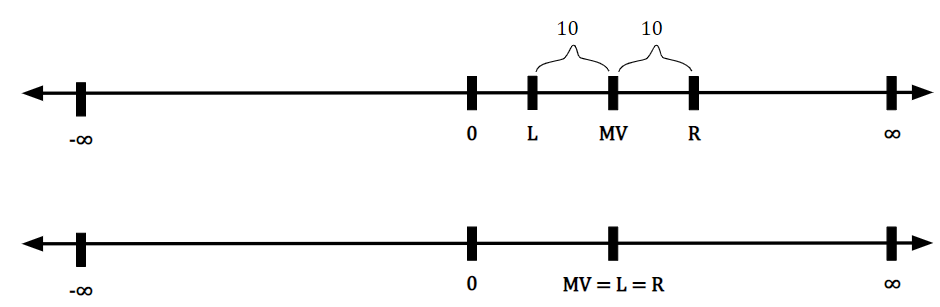
\includegraphics[scale=0.6]{assets/downsian_1.png}
    \end{center}
    Thus, the solution is to get closer to the MV until you converge again. 
\end{itemize}

\subsubsection{Robustness of the Downsian Result}
Even if the parties care about ideology only, they will always both converge on the median voter's preferred policy. Even purely ideological parties have no strategic incentives to propose polarized platforms. 

\bigskip 

The idea is that you still have to care about winning in order to get your policies to pass. Therefore, you will have to keep moving $\epsilon$ closer to the MV than your opponent to win. 

\end{document}